\documentclass[a4paper, 10pt]{article}
\usepackage[utf8]{inputenc}
\usepackage{amssymb}
\usepackage{amsmath}
\usepackage{graphicx}
\usepackage{subcaption}

\title{Object Recognition by Physical Properties Detection using Fault Reconstruction Techniques}
\author{Marco Negrete and Jesús Savage}
\date{RCF-MathWorks Fund - Call 2020\\Technical Report}

\begin{document}
\maketitle
\tableofcontents

\section{Introduction}
\subsection{Motivation}
Consider the following serving-drinks-test scenario: a robot is asked to bring beverages and to do so, the robot performs the following common steps: it navigates to the bar, recognizes the beverages (usually cans or tetra packs), calculate some sort of inverse kinematics, moves its manipulator, grasps the object and returns to the user's location. This is a common situation in @Home tasks, nevertheless, what happens if there are empty cans or tetra packs in the bar? As it is commonly implemented in @Home league, robots are unable to distinguish between empty and full cans, since they commonly rely only in visual information of the beverage containers (see, for example, description papers of last edition winner teams \cite{tdp2019Eindhoven, tdp2019Homer, tdp2019UTS}).
\subsection{Objectives and goals}
The project we propose consist in applying model based fault reconstruction techniques \cite{ding2013model} to estimate the weight of the object being carried by the robot. If we consider the manipulator without load in the final effector as the nominal system, and the weight of the object as an external perturbation causing a faulty behavior, we can apply fault reconstruction techniques to estimate such perturbation, i.e., to estimate object's weight. There are several approaches for MBFR. Residual generation is a common technique where an observer is designed to be sensitive to fault signals. On the other hand, Sliding Mode Observers (SMO) are dynamic estimators designed to be robust against fault signals \cite{shtessel2014sliding}. SMOs also provide the ability to reconstruct the fault signal by filtering the so called output error injection term \cite{alwi2011fault}.
%Mencionar en algun lado quel objetivo del trabajo es la estimacion de la masa del objeto, NO el control de posicion

\section{Background}
\subsection{Sliding Mode Observers}
Sliding mode observers are disticontinuos observers that have the properties of finite time convergence and accurate tracking of the measured states once the sliding surface is reached. These kind of observers can be used to reconstruct faults or disturbance signals through an appropiate filtering of the so-called injection output error. Interested readers can find further information about Sliding Mode Observers in CITE, CITE AND CITE.

Fault detection and isolation, from the control theory approach, is commonly achieved by the implementation of observers that are sensitive to the fault signals. Nevertheless, SMOs inherit the properties of Sliding Modes theory, i.e., SMOs are designed to be robust against disturbances and fault signals and to accurately track the system states. As previously explained, the discontinuos term of the SMO will contain information about the fault signal wich can be reconstructing by obtaining the equivalent output error injection. 

\subsection{Robot Justina's manipulator}
Justina is a domestic service robot built at the Biorobotics Laboratory of the National Autonomous University of Mexico and developed under the ViRBot architecture \cite{savage2008virbot}. This robot and its predecessors have been participating in the Robocup@Home league \cite{wachsmuth2015robocup} since 2006 performing several tasks such as cleaning a table, serving drinks and several other tasks that humans ask for. 

Among other actuators, Justina has two 7-DOF manipulators built with Dynamixel servomotors. Such servomotors allow the user to control them in several forms: by setting a goal position, setting a goal movement speed or setting a desired current which will produce a torque. This latter option is used in this project. Also, these motors provide position sensing with a resolution of less than a tenth of degree. Figure \ref{fig:Justina} shows robot Justina and its sensors and actuators. 
\begin{figure}
  \centering
  \begin{subfigure}[b]{0.35\textwidth}
    \centering
    \includegraphics[width=\textwidth]{Figures/Justina.png}
    \caption{Sensors and actuators.}
    \label{fig:Justina}
  \end{subfigure}
  \hfill
  \begin{subfigure}[b]{0.3\textwidth}
    \centering
    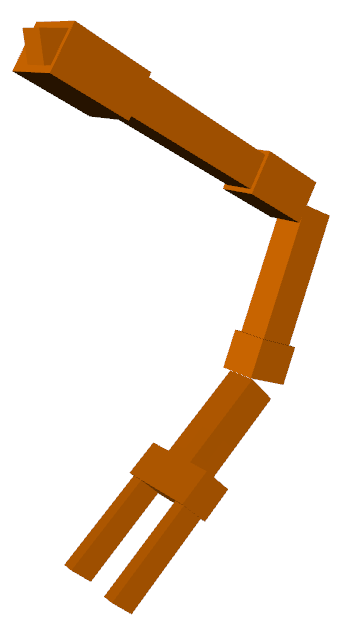
\includegraphics[width=\textwidth]{Figures/left_arm.png}
    \caption{The left manipulator.}
    \label{fig:left_arm}
  \end{subfigure}
  \caption{The domestic service robot Justina.}
\end{figure}

To describe the kinematic chain and some physical properties of the manipulator, we use an URDF file. We already had an URDF describing the whole robot kinematic chain, nevertheless, for this project it was necessary only one of the mainpulators. We chose the left arm and extracted the corresponding tags to a new file. This file was used as a starting point for modeling and simulation purposes. Figure \ref{fig:left_arm} shows the left arm of robot Justina as represented in the URDF.

\section{Mass estimation with Sliding Mode Observers}

\subsection{Dynamic Model}
  From the Langrangian of the manipulator, a dynamic model of the following form can be obtained:
  \begin{equation}
    M(q)\ddot{q} + C(q, \dot{q})\dot{q} + B\dot{q} + G(q) + \Delta(q,\dot{q}, u) = u
    \label{eq:lagrangian}
  \end{equation}
  where $q\in \mathbb{R}^7$ are the joint angles, $M(q)\in \mathbb{R}^{7\times 7}$ is the inertia matrix, $C(q,\dot{q})\in \mathbb{R}^{7\times 7}$ is the Matrix of Coriollis forces, $B\dot{q}\in \mathbb{R}^7$ is the vector of friction forces, $G(q)\in\mathbb{R}^7$ is the vector of gravitational forces, $u$ is the input torque, considered as control signal, and $\Delta(q,\dot{q},u)$ is a vector containing all errors due to uncertanties, disturbances and fault signals.
  
  To design a SMO it is necessary to write the model in variable states form. Let $x_1 = [q_1\;q_2\;q_3\;q_4\;q_5\;q_6\;q_7]^T$ and $x_2 = [\dot{q}_1\;\dot{q}_2\;\dot{q}_3\;\dot{q}_4\;\dot{q}_5\;\dot{q}_6\;\dot{q}_7]^T$ be the state variables. Then (\ref{eq:lagrangian}) can be written as:
  \begin{eqnarray}
    \dot{x}_1 &=& x_2\label{eq:model1}\\
    \dot{x}_2 &=& -M^{-1}(q)\left(C(q, \dot{q})\dot{q} + B\dot{q} + G(q) + \Delta(q,\dot{q},u) - u\right)\label{eq:model2}
  \end{eqnarray}
Equation (\ref{eq:model2} ) can also be written in the form:
  \begin{equation*}
    \dot{x}_2 = f(x_1, x_2, u) + \phi(x_1, x_2, u)
  \end{equation*}
  where $f(x_1, x_2, u) = -M^{-1}(q)\left(C(q, \dot{q})\dot{q} + B\dot{q} + G(q) - u\right) \in \mathbb{R}^7$ is the nominal part and $\phi(x_1, x_2, u) \in \mathbb{R}^7$ contains all terms related to uncertainties, disturbances and fault signals. If the system is correctly identified, and assuming we have no other disturbances than the object being carried, then $\phi(x_1, x_2, u)$ corresponds only to the fault signals, which, in this work, will be caused by the weight of the object being manipulated.

  Thus, if we reconstruct the signal $\phi$ we will be able to estimate the mass of the manipulated object. 

\subsection{Observer for Disturbance Reconstruction}
If a SMO is used to estimate the joint speeds, the unknown term $\phi(x_1, x_2, u)$ in (\ref{eq:model1})-(\ref{eq:model2}) can be reconstructed by an appropriate filtering of the output error injection term. We used the observer proposed by \cite{shtessel2014sliding}:
  \begin{eqnarray}
    \dot{\hat{x}}_1 &=& \hat{x}_2 + z_1\label{eq:observer1}\\
    \dot{\hat{x}}_2 &=& f(x_1, \hat{x}_2, u) + z_2\label{eq:observer2}
  \end{eqnarray}
  where $z_1$ and $z_2$ are the output error injection terms calculated as
  \begin{equation*}z_1 =
    \left[\begin{tabular}{c}
        $z_{11}$\\
        $\vdots$\\
        $z_{17}$
    \end{tabular}\right] = 
    \left[\begin{tabular}{c}
        $\lambda\vert q_1 - \hat{q}_1\vert ^{1/2}sign(q_1 - \hat{q}_1)$ \\
        $\vdots$\\
        $\lambda\vert q_7 - \hat{q}_7\vert ^{1/2}sign(q_7 - \hat{q}_7)$
    \end{tabular}\right]
\end{equation*}
\begin{equation*}z_2 =
  \left[\begin{tabular}{c}
      $z_{21}$\\
      $\vdots$\\
      $z_{27}$
    \end{tabular}\right] = 
  \left[\begin{tabular}{c}
      $\alpha sign(q_1 - \hat{q}_1)$ \\
      $\vdots$\\
      $\alpha sign(q_7 - \hat{q}_7)$
    \end{tabular}\right]
\end{equation*}

In this observer, the sliding surface is given by $\sigma = x_2 - \hat{x}_2$. When the sliding mode is reached, it holds that:
\[\sigma = \dot{\sigma} = \dot{x}_2 - \dot{\hat{x}}_2 = f(x_1, x_2, u) + \phi(x_1, x_2, u) - f(x_1, \hat{x}_2, u) - z_{2_{eq}} = 0\]
Since,  $x_2 = \hat{x}_2$, then
\begin{equation}
  z_{2_{eq}} = \left[\begin{tabular}{c}
      $z_{21_{eq}}$\\
      $\vdots$\\
      $z_{27_{eq}}$
    \end{tabular}\right] = \phi(x_1, x_2, u) =
  \left[\begin{tabular}{c}
      $\phi_1(q_1,\dots, q_7, \dot{q}_1, \dots, \dot{q}_7, u_1, \dots,u_7)$\\
      $\vdots$\\
      $\phi_7(q_1,\dots, q_7, \dot{q}_1, \dots, \dot{q}_7, u_1, \dots,u_7)$
    \end{tabular}\right]
  \label{eq:zeq}
\end{equation}
where $z_{2_{eq}}$ is the equivalent output error injection which can be obtained by an appropriate low-pass filtering of $z_2$.

Noisy and low sampling frequency rates can cause big chattering effects on the estimated states. This is not a problem, since the output error injection will be low-pass filtered, nevertheless, if estimated states are used for a closed-loop control, then actuator signals will have high frequency components that will result in hardware damage. Thus, as it will be later discussed, the SMO is used to estimate the fault signal but, to implement a closed-loop control, an Extended Kalman Filter is used instead. 

\subsection{Mass estimation}
The term $\phi(x_1, x_2, u)$ in equation (\ref{eq:model2}) is a function of input torque, joint positions and joint speeds. The mass of the object could be calculated in any point of the state space, nevertheless, calculations are much simpler if such estimation is made only when the manipulator is in a constant position. If $\dot{q}= \ddot{q} = 0$, then $\phi(x_1, x_2, u) = \phi(q)$ depends only on the gravitational torques caused by the weight of the object being carried. From (\ref{eq:model2}) we can see that disturbance $\phi$ is a signal of acceleration, not a torque signal. Let $\tau_o = [\tau_o1,\dots,\tau_o7]^T$ be the torque exerted by the manipulated object with mass $m_o$ and weight $w_o=m_o g$ on each joint. Vector $\tau_o$ can be obtained by multiplying signal $\phi$ by the inertia matrix $M(q)$. Thus, from equation (\ref{eq:zeq}):

\begin{equation}
  \tau_o = M(q)\phi(q) = M(q)z_{2_eq}
  \label{eq:taus}
\end{equation}

Figure \ref{fig:taus} shows torques $\tau_o$ on the different joints. Torques are zero where the weight force is applied along the axis of rotation. In figure \ref{fig:taus} this is the case for joints $O_3$, $O_5$ and $O_7$.
\begin{figure}
  \centering
  \begin{subfigure}[b]{0.4\textwidth}
    \centering
    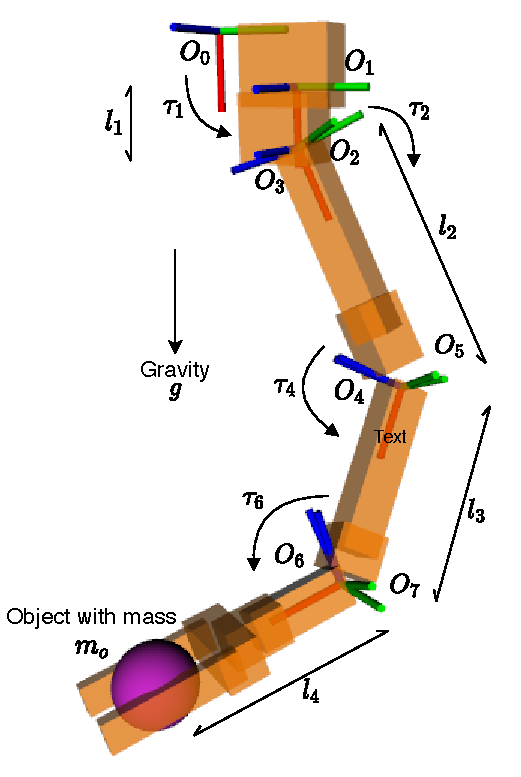
\includegraphics[width=\textwidth]{Figures/fault_torques.pdf}
    \caption{Torques $\tau_o$ on each joint.}
    \label{fig:taus}
  \end{subfigure}
  \hfill
  \begin{subfigure}[b]{0.55\textwidth}
    \centering
    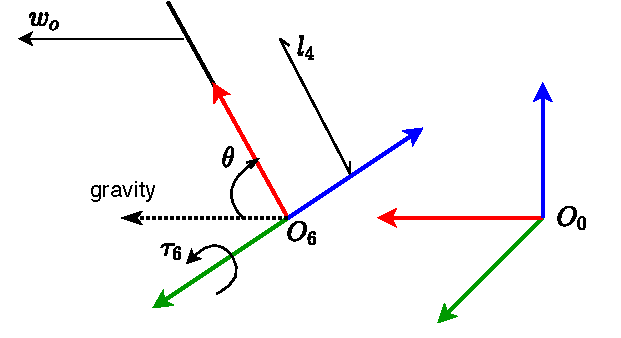
\includegraphics[width=\textwidth]{Figures/RPY.pdf}
    \caption{Calculation of $m_o$ from $\tau_6$.}
    \label{fig:rpy}
  \end{subfigure}
  \caption{Variables and frames to calculate $m_o$.}
\end{figure}

Torques $\tau_o$ are caused by the weight of the object being carried and thus they can be obtained in a form similar to term $G(q)$ in model (\ref{eq:lagrangian}). The mass $m_o$ can be estimated from any component of $\tau_o$, nevertheless, due to the kinematic configuration, it is much easier if we use torque on joint $O_6$.

Consider the figure \ref{fig:rpy}. The frame $O_6$, attached to joint 6, is the frame $O_0$ translated and rotated. To represent the rotation we used the Roll-Pitch-Yaw angles $(\rho, \theta, \psi)$. As it can be seen, the weight $w_o=m_o g$ causes the torque $\tau_6=-m_o g l_4 \sin\theta$ and the mass of the manipulated object can thus be calculated as:
\begin{equation}
  m_o = -\frac{\tau_6}{gl_4\sin\theta}
  \label{eq:mass}
\end{equation}
where $\theta$ is the \textit{pitch} angle of frame $O_6$ w.r.t. $O_0$, $g$ is the gravity acceleration, $\tau_6$ is the disturbance torque calculated according to (\ref{eq:taus}) and $l_4$ is the distance from joint $O_6$ to the center of mass of the manipulated object. As it will be latter explained, errors in the estimation of $l_4$ will cause proportional errors in the estimation of $m_o$.

Note that when $\theta=0$ it is not possible to estimate $m_o$ because $\theta=0$ means that the manipulated object is ``hanging'' from the joint and its weight is not exerting any torque on the joint. There are two possible ways overcome this situation: use another disturbance $\tau_i$ or moving the manipulator to a useful position. Second option is more feasible since the relation between $w_o$ and $\tau_i$ becomes more complex in the rest of the joints. 

\subsection{Extended Kalman Filter}
Sliding Mode Observer have the great advantage of being robust against disturbances, nevertheless, due to the discontinuos ouput error injection, they can have high frequency components in the estimated states. SMOs are useful for fault reconstruction but, due to the noise and low frequency sampling rate, it is better to use an Extended Kalman Filter (EKF) as part of the closed-loop control strategy.

From (\ref{eq:model1})-(\ref{eq:model2}), we have the state transition model for the noisy system:
\begin{eqnarray}
    \dot{x}_1 &=& x_2 + \nu_1\label{eq:noisymodel1}\\
    \dot{x}_2 &=& f(x_1, x_2, u) + \phi(x_1, x_2, u) + \nu_2\label{eq:noisymodel2}
\end{eqnarray}
where $\nu \in\mathbb{R}^14$ is a vector of noise signals without temporal correlation, zero mean and covariance matrix $Q\in\mathbb{R}^{14\times 14}$. Remember that system state variables are the seven joint positions and seven joint speeds.

In this work, since we are measuring the joint positions, our observation model is:
\begin{equation}
  z = h(x,u) + \omega = [q_1,\dots,q_7]^T + \omega
  \label{eq:obsmodel}
\end{equation}
where $\omega\in\mathbb{R}^7$ is Gaussian noise without temporal correlation, zero mean and covariance matrix $R\in\mathbb{R}^{7\times 7}$.

Chosing between the cotinuous or discrete version of the EKF depends on the frequency sampling. In this work we achieved a sampling of 250 Hz, which is much faster than the system dynamics, but too slow for a SMO. Also, since Simulink provide tools for continuos controls, we chose the continuos version of the EKF:
\begin{eqnarray}
  \dot{\hat{x}}_1 &=& \hat{x}_2 + K_1 y_1 \label{eq:ekf1}\\
  \dot{\hat{x}}_2 &=& f(\hat{x}_1, \hat{x}_2, u) + K_2 y_2\label{eq:ekf2}\\
  \dot{P} &=& FP + PF^T - KRK^T + Q\label{eq:ekf3}
\end{eqnarray}

where $y=z - \hat{x}_1$ is the error between the estimated and measured outputs, $F$ is the Jacobian of the state transition model and $K$ is the Kalman Gain calculated as:
\[
K = PH^TR^{-1}
\]
with $H\in\mathbb{R}^{7\times 14}$, the Jacobian of the observation model, which, in this case, is the constant matrix:
\[
H = \left[0\quad I_7\right]
\]
Note that in (\ref{eq:ekf2}) we are using only the nominal part of the system and thus, if $\phi\neq 0$ (i.e., if an object is being manipulated), the estimated states will not converge to the real states. Since estimated states are used for position control, such estimation error will cause a steady state error in the controller. This is in principle undesirable, nevertheless, we can tolerate this error since the main goal of this work is the estimation of the mass, not the performance of the controller. Calculations to estimate $m_o$ are made under the assumption that the manipulator is in a constant position, thus, driving the manipulator to a constant $q_f$, although slightly different from the desired $q_g$, is a good enough performance for the control-observation loop. 
\subsection{Position control}
As stated before, equations for estimating $m_o$ are derived under the assumption that the manipulator is in a constant configuration. We implemented a PD+Gravity controller using the EKF estimated states:

\begin{equation}
  u = G(\hat{q}) + K_p(q_d - \hat{q}) + K_d(\dot{q}_d - \hat{\dot{q}})
\end{equation}

where $\hat{q}$ and $\hat{\dot{q}}$ are the filtered measured positions and EKF-estimated speeds, respectively; $G(\hat{q})$ is the vector of gravity torques of the nominal part of the model (no noise and no fault signals) and 

As explained in the previous section, when the manipulator takes an object, the estimated states do not converge to the real ones and then the controller shows an steady state error.

MENCIONAR AQUI LO DEL POLINOMIO DE 5TH GRADO

\section{System Identification}

\section{Simulink implementation}
The Sliding Mode Observer is a copy of the system plus an output error injection term, with the form:
  \begin{eqnarray}
    \dot{\hat{x}}_1 &=& \hat{x}_2 + z_1\label{eq:observer1}\\
    \dot{\hat{x}}_2 &=& -M^{-1}(q)\left(C(q, \dot{\hat{q}})\dot{\hat{q}} + B\dot{\hat{q}} + G(q) - u\right) + z_2\label{eq:observer2}
  \end{eqnarray}
  The nominal part can be derived from the lagrangian, nevertheless, the analytic form is too complex due to the number of DOF. Instead, we used the numeric solution provided by the Simulink Robotics Toolbox, as shown in figure:
  \begin{figure}
    \centering
    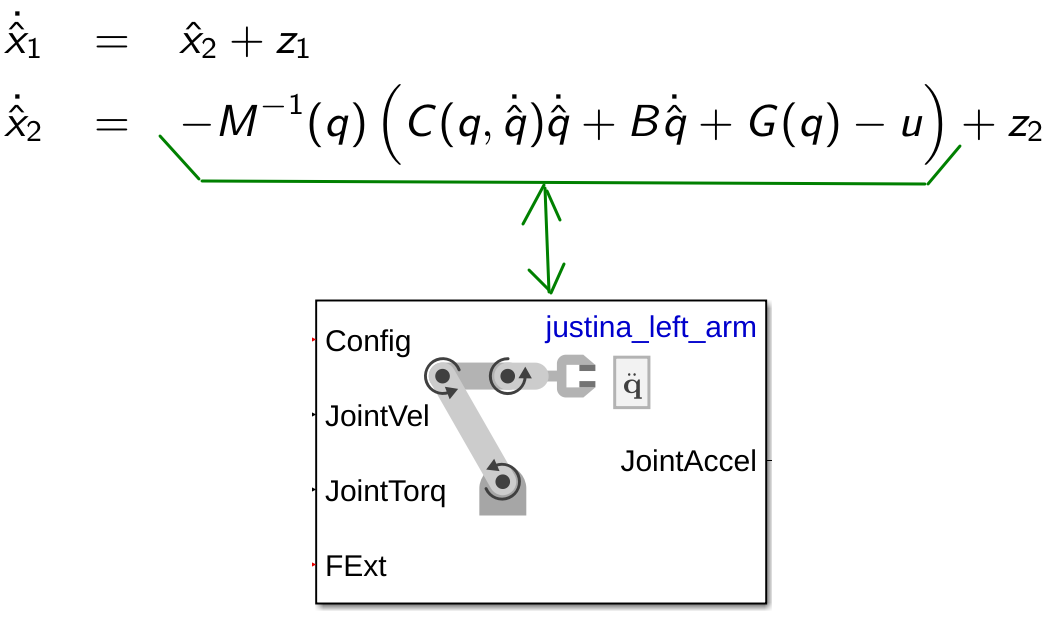
\includegraphics[width=0.5\textwidth]{Figures/SMOwithSimulink.png}
  \end{figure}

  Also, from equation (\ref{eq:Mqz}), it is necessary to compute the inertia matrix $M(q)$ to obtain the perturbing torques $\phi$. Similar to the observer, instead of obtaining the algebraic expression of $M(q)$, we used the numeric calculation provided by the Robotics Toolbox:

\subsection{Quantization of input torque and position measurements}
To achieve a simulation more similar to the conditions of the real manipulator, we added a quantization for input torque and position measurements. Dynamixel motors can read position with 12 bit resolution and can set torque with 10 bit resolution. The implemented simulation add this quantization effect, which is shown in figures ASDFASF and ASDFSAFS. 
\textbf{Agregar grafica con mucho zoom donde se vean escalonadas las posiciones y los torques. }

\subsection{A ROS node for each task}

\section{Simulation results}
\subsection{Joint speed estimation in finite time}

\subsection{SMO performance with low sampling rate}

\subsection{SMO performance with noisy measurements}

\subsection{Mass estimation}

\subsection{Effects of uncertanties in physical parameters}

\subsection{Effects of object position along gripper}

\section{Experimental results}

\section{Reusability}

\section{Conclusions}
Se utilizó software de matlab para poder calcular la parte nominal del modelo dinámico para el brazo de 7 dof que de otro modo hubiera sido muy difícil de calcular debido a la complejidad del sistema

\bibliographystyle{abbrv}
\bibliography{References}
\end{document}
